\label{chip}
\begin{titlepage}

\section{Pixel carateristics}
Fanno parte dei detector a semiconduttore
\begin{itemize}
\item puoi fare giunzioni di che tipo,
\item backprocess,
\item come fai isolation?
\item cos'è il puncht.?
\item Info sull'inversione e qualcosa sulla radiazione?!
\item carica nel substrato in funzione dell'energia persa: due conti con MIP e assorbimento totale
\end{itemize}

Pixel detector can provide informations about both the cordinates in the plane; that is by
construction, but with some strategy, as positioning them with a stareo angle, even
the third cordinate can be measured. SPIEGARE?\\
Because of their dimension\footnote{Their size is not limited by bump-bonding technique,
as happens instead for hybrid pixels} (this is an advantage $\sim$
30 $\mu m$ or even better) and then their spatial resolution
($\sim$ 5-10 $\mu m$) they have fastely been used in the inner layer of accelerator
experiments as vertex detector.\\
Talking about resolution, if only a binary information is read (pixel fired if hit
and 'spento' if not), the spatial resolution of a single hit is:
\begin{equation}
\sigma_x = \frac{p}{\sqrt{12}}
\end{equation}
where $p$ is the pitch between pixels.
To improve the position resolution of a single hit one can use other analogical
informations; for example, a standard tecnique also used in multiwire chambers and
in strip detectors, is the capacitive charge division.\\
\begin{itemize}
\item capacitive charge division
\item Morover they can be used as beam monitor???
\end{itemize}

\subsection{Monolitic active pixel}
Monolitic active pixel acoomodate on the same wafer both the sensor and the front
end electronics.\\
They have been first proposed and realized in 1990s and their use has been enabled
by the development of the electronic sector which guarantees the decrease in CMOS
dimension, as stated by the Moore's law\footnote{Moore's law states that logic
density doubles every two years.}.\\
As a matter of fact the dimension of componenents, their organization on the
pixel area and logic density are hot topics for the designers of this type of detector
and for all high rate experiments who intend to use pixel deterctor; typiccally
different decisions are taken for different purposes. \\
Collegato al fattore spazio c'è ad esempio la disponibilità di integrare sul pixel un trigger.
Questo è un argomento caldo per l'utilizzo di questi detector in rivelatori di esperimenti
agli acceleratori ad esempio; ne parlerò dopo.

Moreover one other benefit related with the possibility of using the microelectronics
and CMOSS in digital circuit is the lack of resistors, which require a lot of
space and have a high power consumption, in favor of MOSFET transistors, whose power
consumption depends by the switching frequency\footnote{Discorso fatto con Ludovico
sul fatto che i CMOSS tirano meno rispetto al circuito analogico}.
Scrivi perchè si usano i CMOSS invece dei transistor: discorso sulla potenza e sull'
elettronica digitale.
\begin{itemize}
\item discorso dei CMOSS
\end{itemize}

\subsubsection{MAPS and DMPAS}
Monolithic active pixel can be distinguish beteween two main category: MAPS and depleted
MAPS (DMAPS).

MAPS (figure \ref{fig:MAPS_scheme}) have typically an epilayer in range between 1-20 $\mu m$ and because they
are not depleted, the charge is mainly collected by diffusion rather then by drift.
This makes the path of charges created in the bulk longer than usual and then they are
slow (of order of 100 ns) and the collection could be partial expecially after
an irradiation of the detector, when the trapping probability become highter.

\begin{figure}
\centering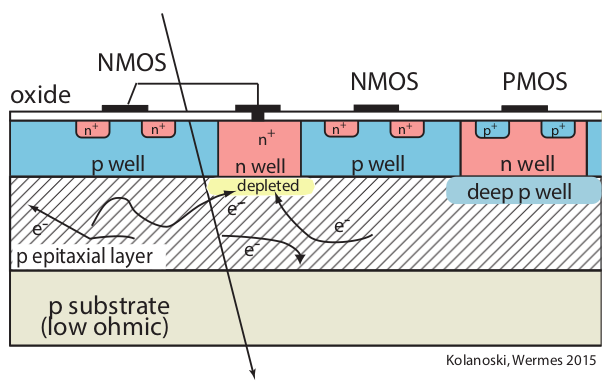
\includegraphics[width=8cm]{figures/MAPS_scheme.png}
\caption{Concept cross section of one MAPS pixel}
\label{fig:MAPS_scheme}
\end{figure}
\begin{figure}
\centering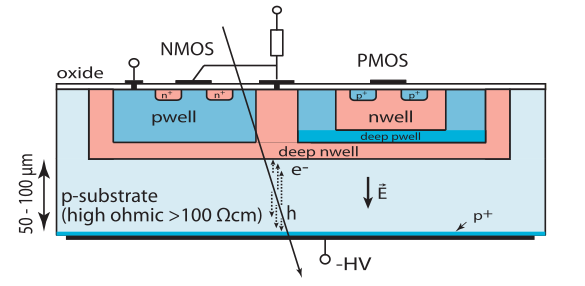
\includegraphics[width=9cm]{figures/DMAPS_scheme.png}
\caption{Concept cross section of one DMAPS pixel}
\label{fig:DMAPS_scheme}
\end{figure}

DMAPS (figure \ref{fig:DMAPS_scheme}) are istead depleated (depleted region underneath
the collection electrode is typically 15-25 $\mu$m thick) and depending on the
bias applied $V$ and on the resistivity of the bulk $\rho$ the depleated region
$d$ ($\sim$ 25-150 $\mu m$) is: (vedi a pag 283 del KW)
\begin{equation}
   d \propto  \sqrt{ \rho V}
\end{equation}
Looking at this formula one could think that high resistivity\footnote{Hight resistivity
crystall can be produces using Czochralki (Cz) or float-zone (Fz) process;
the fist one creates a silicon bulk with a highter oxygen concentration
which can be beneficial for radiation damage} bulk are prefered, but
instead for high radiation applications the starting resistivity is not too crucial
and lower resisistivity may be advantageous (pag 37 review).\\

The main drawback of DMAPS is a new capacity term that contributes to the total
amplifier input capacity; in addition to th capacity between pixels ($C_{pp}$) and
between the pixel and the backside ($C_{b}$), a non negligible contribution comes
from the capacities between wells ($C_{SW}$ and $C_{WW}$) needed to shield the
embedded electronics.\\
These capcaities affect the thermal and 1/f noise of the charge amplifier and
the $ \tau_{CSA}$ too.\\

\begin{figure}
\centering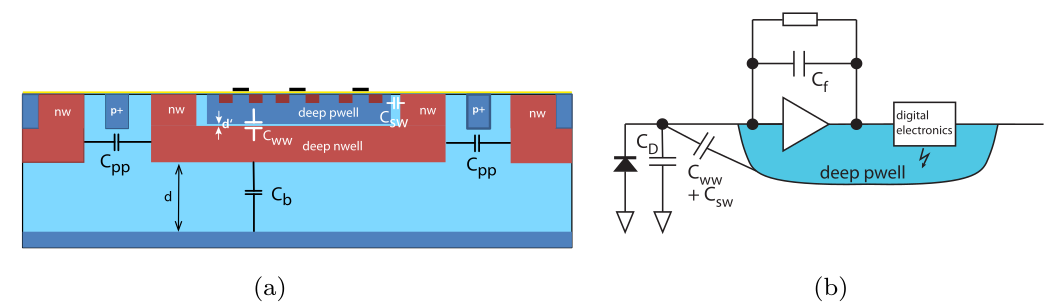
\includegraphics[width=12cm]{figures/DMAPS_capacity.png}
\caption{$C_{pp}$, $C_{b}$, $C_{WW}$, $C_{SW}$}
\label{fig:DMAPS_capacity}
\end{figure}

There are two different sensor-design approaches (figure \ref{fig:large_small_sensor_scheme})
to DMAPS:
\begin{itemize}
\item large fill factor: a large collection electrode that is a large deep n-well
 and that host the embedded electronics
\item small fill factor: a small n-well is used as charge collection node
\end{itemize}

one with a large fill factor, and so with a large sensor, and the other
with a small electrode.

Larger charge collection electrode sensors means uniformity of electric field in
the bulk, and so shorter drift path and less trapping. The drawback is the large
capacity (???) and, as I have just explained, this contributes to the noise, to a
speed penalty and possible cross talk.
On the other hand the small electrode variant has a small collection node, that means
it has a small capacity (5-20 fF), e quindi tau più brevi e minor potenza dissipata,
however il campo elettrico può essere disuniforme and this means again
that the path percorso by drift by particles is longer and then this
detectors suffers radiation. \\
These two different types of sensor require different amplifier (section \ref{sec:}).

\begin{figure}
\centering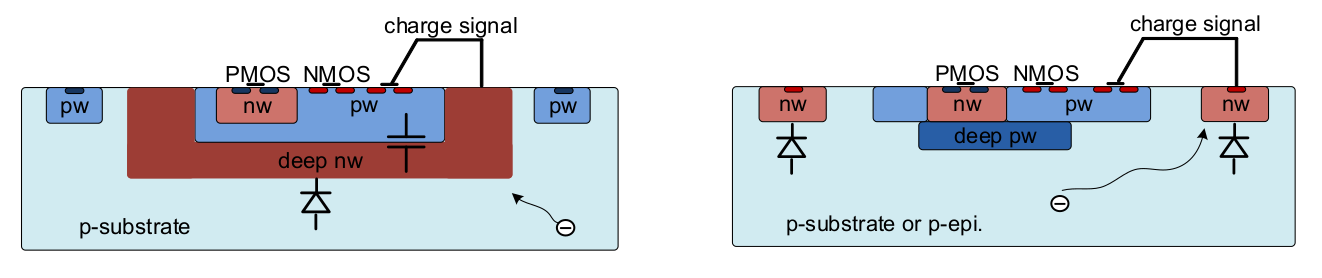
\includegraphics[width=12cm]{figures/large_small_sensor_scheme.png}
\caption{Concept cross section with large and small fill factor}
\label{fig:large_small_sensor_scheme}
\end{figure}

\begin{table}
\begin{center}
\begin{tabular}{|c | c |c |}
\hline
& small fill factor & large fill factor\\
\hline
\hline
small sensor C & $\surd$ ($<$ 5 fF) & $\times$ ($\sim$ 100-200 fF)\\
low noise & $\surd$ & $\times$\\
low cross talk & $\surd$ & $\times$ \\
velocity perfomances & $\surd$ & $\times$ ($\sim$ 100 ns)\\
short drift paths & $\times$ & $\surd$ \\
radiation hard & $\times$ & $\surd$ \\
\hline
\end{tabular}
\caption{Small and large fill factor DMAPS characteristics}
\label{tab:DMAPS_large_small_fillfactor}
\end{center}
\end{table}

\subsection{Analog front end (AFE)}
Dopo che la carica è stata creata nel substrato e abbia driftato fino agli elettrodi
inducendo un segnale su questi utlimi, il segnale creato entra nel circuito di FE
(figure \ref{fig:readout_scheme}).

\begin{figure}
\centering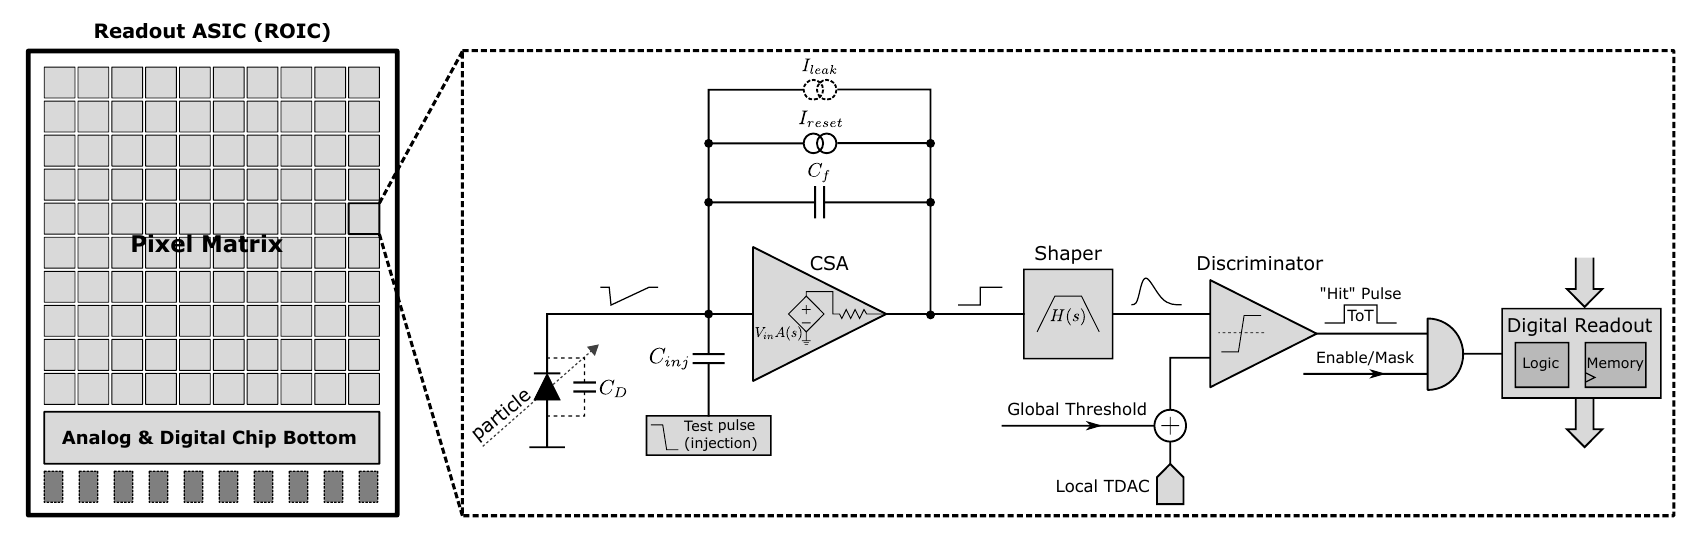
\includegraphics[width=15cm]{figures/readout_scheme.png}
\caption{Readout FE scheme}
\label{fig:readout_scheme}
\end{figure}

One of the most important specification to minimize the noise is whether the preamplifier
(that actually is the only amplification step) is as close as possible to the sensor contact.\\
The preamplifier needs a reset to the baseline mechanism and a way to discharge
the feedback capacitor; this step is often trained by a costant current reset circuit.
VANTAGGI DEI VARI MODI DI FARE RESET (POI QUANDO PARLI DEI FE DI ARCADIA FAI RIFERIMENTO A QUESTA COSA).

The shaper is usually a band-pass filter whose $\tau$ time costant is tuned in
order to optimize S/N ratio and pilanzie-up too.\\

Last but not least, even better it probably is the main step of the reaout chain
expecially if only binary information is stored (1 = pixel hit, 0 = pixel don't hit),
there is the discriminator; his importance is due to the fact that its threshold
is the easiest parameter to set and change, and it has an obvious direct impact
on the output data stored.\\

\subsubsection{Preamplifier}
Even if circuits on the silicon crystal are only costruct by CMOSS, a
preamplifier can be modellized as an operational amplifier (OpAmp) with an impedence
feedback (first step in figure \ref{fig:readout_scheme}).\\
Depending on whether a capacity or a resistance is used as feedback, respectevely,
a charge or a voltage amplifier is used (figure \ref{fig:amplifier}).
\begin{figure}
\centering\includegraphics[width=15cm]{figures/.png}
\caption{Amplifier}
\label{fig:amplifier}
\end{figure}
The amplification gain is determined by the input and feedback impedance:
\begin{equation}
G = \frac{v_{out}}{v_{in}} = \frac{Z_{f}}{Z_{in}}
\end{equation}

If the signal duration is longer than the charateristic time ($R_SC_D$) of the amplifier with
a resistor in feedback ($\tau << \Delta t$), then the second condition in equation \ref{eq:} is satisfied
and the system operates as a current amplifier:
\begin{equation}
v_{out} = \frac{R_f}{R_S}v_{in}(t) = R_{f}i_{S}(t)
\end{equation}

When the S/N is small a charge amplifier is prefered.

\begin{equation}
v_{out}(t) = -a_{0}v_{in}(t) = 


\end{eqution}


If the voltage input signals are large enought and have a sharp rise time, the voltage
sensistive preamplifier is often used. For this reason this preamplifier don't
perfectely suit to semiconductor detectors, especially for that one with large capacity
that also have large fill factor ($v_{in} = Q/C_{D} \approx$ 3fC/100 pF = 0.03 mV); on the other hand they are fine for that one with
very low capacity ($v_{in} = Q/C_{D} \approx$ 3fC/3 pF = 1 mV).

\subsubsection{Noise source}
It is important to establish the noise source of MOSFET (Metal Oxide Semiconductor Field
Effect Transistor) which are made by CMOSS blocks.\\
It is usefull to express the noise contributions as " voltage series" and "current parallel"
(with the input amplifier gate) noise.\\


Tipi di rumore del preamplificatore.

One of the main problems of MAPS is the cross talk: one speaks about cross talk
when an input signal causes an output signal on neighbouring electrodes; digital signals
in the FE electronics do a lot of oscillations and digital switching produce spikes
and so noise.\\
METTI FORMULA DEL CROSS TALK E FAI VEDERE CHE PIÙ C È PICCOLA E MENO CROSS TALK HAI.\\
A way to partially reMETTI FORMULA DEL CROSS TALK E FAI VEDERE CHE PIÙ C È PICCOLA E MENO CROSS TALK HAI.\\
solve the problem, the analogical and digital part have different
bias channels and also the buses to MASS are different: this tecnique reduces the
loop in the circuit and therefore the induces singlas.\\


\subsection{Readout logic}
To store the analogical informations (charge collected, evolution of signal in time)
big buffers and a big bandwidth are needed.
Digital information, instead, means that if one pixel is hit 1 is recorded, and if
not 0 is recorded.\\
Typically one want to save some more information than the digital one, but also
less then the analogical one, so one choise used in some design is to save the time over threshold
(ToT) of the pulse; this is a a relatively coarse information (about 7 bits) but it
is correlated with the deposited charge by the impinging particle in the detector.

This is why, while the front end architecture remains similar from one generation
to the next (almost all pixels have a FE-ALPIDE), the processing of the information
produced by the front end, and the relationship of the front end to the rest of
the chip, changed significantly.\\
Il modo con cui vengono lette le hit su una matrice è il column drain readout.\\
The simple 3T (three transistor) readout has a row select, a
source-follower buffer and an input baseline reset;

Moreover the readout architetcture can be full, if every hit from every pixel must eventually
make its way to the data output, or triggered, if hits are recorded during a trigger signal.
Again, on the one hand the triggered-readout needs buffers and storage memories
(therfore needs space on the pixel are to accomodate them), on the other the full readout,
because there is no need to store hit data on chip, needs an high enough bandwidth.\\
I will now give some hints about the optimization between this two trends.

If all the pixels in a column share a data bus to the EoC and only one pixel at a time can
be use and there aren't any storage memory, the column (si comporta) as a single
server queue and the probability for waiting a time greater than $t$ with an input
hit rate $\mu$ in a column and an output bandwidt $B_W$ is:
\begin{equation}
P(T > t) = \frac{\mu}{B_W} e^{-( B_W-\mu )t}
\end{equation}
To avoid hit loss (let's neglect the contribution to the inefficency of the dead
time $\tau$), for example imponing $P(T > t)\sim$0.001, one obtains
$(B_W -\mu)t_t\sim$6, where $t_t$ is the time to transfer the hit;
since $t_t$ is small, one must have $B_W \gg \mu$, that means a high bandwidth.

If shift registers (SR) are used to transfer data instead of buses the bandwidth $B_W$
of the SR corresponds to the clock speed; differently from the bus case, each pixel
sees a different bandwidth depending on the position on the queue: the first pixel
in the priority logic chain , that is the closest pixel to the EoC typically,
sees a full bandwidth, but the next pixel sees less bandwidth because
occasionally it will be blocked by data from the previou pixel.\\
Then the condition about the bandwidth and the hit rate become: $B_{W,i} > \mu_{i}$,
where the index $i$ means the requirement is for a single pixel. If all the pixels
on the same column
have the same rate $\mu = N\mu_{i}$ and the condition become $B_{W} > \mu$.
The bandwidth must be chosen such that the mean time between hits of the last pixel
in the readout chain is bigger than that.\\
Questa condizione tra banda e rate sulla colonna ci dice già una cosa importante:
il fatto che l'algoritmo di lettura column drain non è scalabile: infatti se aumento
il numero di pixel sulla stessa linea di lettura rischio di violare la condizione.\\
La scalabilità risiede quindi nel poter utilizzare tanti chip piccoli.\\


If instead the hits are stored in buffers until a trigger signal arrives, the input rate
to column bus is reduced as $\mu'=\mu t$, where $t$ is the trigger rate.
This implies that $B_{W} \gtrsim \mu'$, that is a very relaxed condition on the
bandwidth, but the limiting factor is the amount of memory  which the pixel area
can host; the amount needed depends on the trigger frequency 1/$t$ as
$\propto\mu/t$, that means that the highter the trigger frequency and the highter
the hit rate that can be handled. \\
In order to have an efficient use of memory on pixel area it's convenient
grouping pixels into regions with shared storage. Let's look what happens when
single pixel local storage is used: for example, suppose to have a 50 kHz single
pixel hits rate and a trigger frequency of 1/5 microseconds, allora il rapporto dei due
è 0.25 e cioè il numero medio di hit perse per trigger signal.\\
usando la statistica di Poisson, uno dovrebbe storare 3 hit per pixel se volesse
raggiungere il 99.9 per cento di efficienza.\\
Consideriamo cosa succede se faccio un gruppo di quattro pixel: allora se il rate
medio di 1 hit sui 4 pixel (sempre 50 khz di single pixel) per ogni trigger signal, allora se volessi un'eff di 99.9
avrei bisogno di un buffer depht of 5 region-hits. Quindi significa che in media per
ogni pixel avrei 5/4 = 1.25 buffer depht, minore di quello di prima.\\
L'architettura di lettura che colloca i pixel in regioni da 4 si chiama FE-I4.\\

One standard way to reduce the readout bandwidth is to implement the zero suppression
on the pixel: only informations about channels with an hit (when signal exceeds
the discriminator threshold) are read.

Per gli esperimenti agli acceleratori, e soprattutto per gli esperimenti che
intendono aumentare la luminosita, è sicuramente di particolare importanza
l'occupancy dei pixel: sia il rate del noise va mantenuto basso, sia un
bisogna prestare attenzione al pile up.
L'occupancy tra le altre cose dipende dalla differenza tra threshold e offset del
segnale, per cui uno può agire sulla soglia per poterla cambiare.\\
FORMULA? slide APSEL\\
Una soluzione potrebbe essere mettere un trigger e in sincro con il beam mettere
il reset avviene ad ogni beam collision; questo consuma però un sacco di power. \\


\end{titlepage}
